\section{Appendix}
\label{sec:Appendix}

\begin{table}[h!]
    \centering
      \begin{tabular}{ |p{2cm}||p{2cm}||p{2.9cm}|p{1.9cm}|p{1.7cm}|p{1cm}|p{1.2cm}|  }
        \hline
        \multicolumn{7}{|c|}{Evaluation Individual Regressors} \\
        \hline
        Model & Scaler & RMSE / €  & MSE / €  & MAE / € & $ \mathrm{R}^2 $& TT / s\\
        \hline
        \multirow{4}{2cm}{XGBoost (Tree)} & Standard & $2400.5 \pm  429.7$ & $4557951.9$ & $1350.6$ & $0.894$ & $2.37$\\
        & \cellcolor[HTML]{FFFACD} Gaussian  & \cellcolor[HTML]{FFFACD} $2379.3 \pm  395.6$ & $4514569.4$ & \cellcolor[HTML]{FFFACD} $1352.1$ & \cellcolor[HTML]{FFFACD} $0.897$ & $2.42$\\
        & Robust & $2405.0 \pm  425.2$ & $4500529.4$ & $1356.1$ & $0.895$ & $2.71$\\
        & No Scaling & $2389.3 \pm  415.9$ & $4479635.3$ & $1342.4$ & $0.897$ & $2.35$\\
        \hline  
        \multirow{4}{2cm}{XGBoost (Linear)} & Standard & $3438.8 \pm  488.6$ & $8740382.4$ & $1920.3$ & $0.783$ & $2.37$\\
        & Gaussian  & $3349.4 \pm  348.1$ & $9572071.3$ & $2082.5$ & $0.765$ & $2.45$\\
        & Robust & $3460.8 \pm  500.0$ & $8402075.3$ & $1915.2$ & $0.787$ & $3.43$\\
        & No Scaling & $3444.1 \pm  498.6$ & $9371909.1$ & $2027.9$ & $0.764$ & $2.54$\\
        \hline  
        \multirow{4}{2cm}{CatBoost} & \cellcolor[HTML]{98FB98} Standard & \cellcolor[HTML]{FFFACD} $2334.1 \pm  386.9$ & $4146873.1$ & \cellcolor[HTML]{FFFACD} $1297.3$ & \cellcolor[HTML]{FFFACD} $0.902$ & $2.15$\\
        & Gaussian  & $3460.8 \pm  500.0$ & $4407888.2$ & $1320.6$ & $0.899$ & $1.73$\\
        & Robust & $2343.9 \pm 395.1$ & $4174227.2$ & $1305.9$ & $0.899$ & $2.51$\\
        & No Scaling & $2310.0 \pm  417.6$ & $4148775.5$ & $1300.4$ & $0.901$ & $1.81$\\
        \hline
        \multirow{4}{2cm}{AdaBoost} & Standard & $3583.1 \pm  440.2$ & $10952648.3$ & $2337.3$ & $0.768$ & $2.62$\\
        & Gaussian  & $3540.2 \pm  427.0$ & $11411895.8$ & $2325.4$ & $0.767$ & $2.54$\\
        & Robust & $3650.5 \pm 421.2$ & $11127472.7$ & $2370.4$ & $0.762$ & $3.22$\\
        & No Scaling & $3626.5 \pm  463.8$ & $11975364.1$ & $2421.71$ & $0.751$ & $2.86$\\
        \hline   
        \multirow{4}{2cm}{Extra Trees} & Standard & $2494.6 \pm  407.3$ & $4481129.5$ & $1349.5$ & $0.889$ & $3.47$\\
        & Gaussian  & $2507.0 \pm  391.9$ & $4426545.2$ & $1357.3$ & $0.886$ & $3.47$\\
        & \cellcolor[HTML]{FFFACD} Robust & \cellcolor[HTML]{FFFACD} $2470.0 \pm 408.5$ & $4394657.3$ & \cellcolor[HTML]{FFFACD}$1339.0$ & \cellcolor[HTML]{FFFACD}$0.890$ & $3.76$\\
        & No Scaling & $2517.8 \pm  435.9$ & $4590153.2$ & $1369.7$ & $0.891$ & $3.94$\\
        \hline
      \end{tabular}
      \caption{RMSE, MSE, MAE, $R^2$ score and training time for all individual models and applied scaling methods. The best-performing values are highlighted.}
      \label{tab:Metrics}
\end{table}

\begin{figure}
    \centering
        \centering
        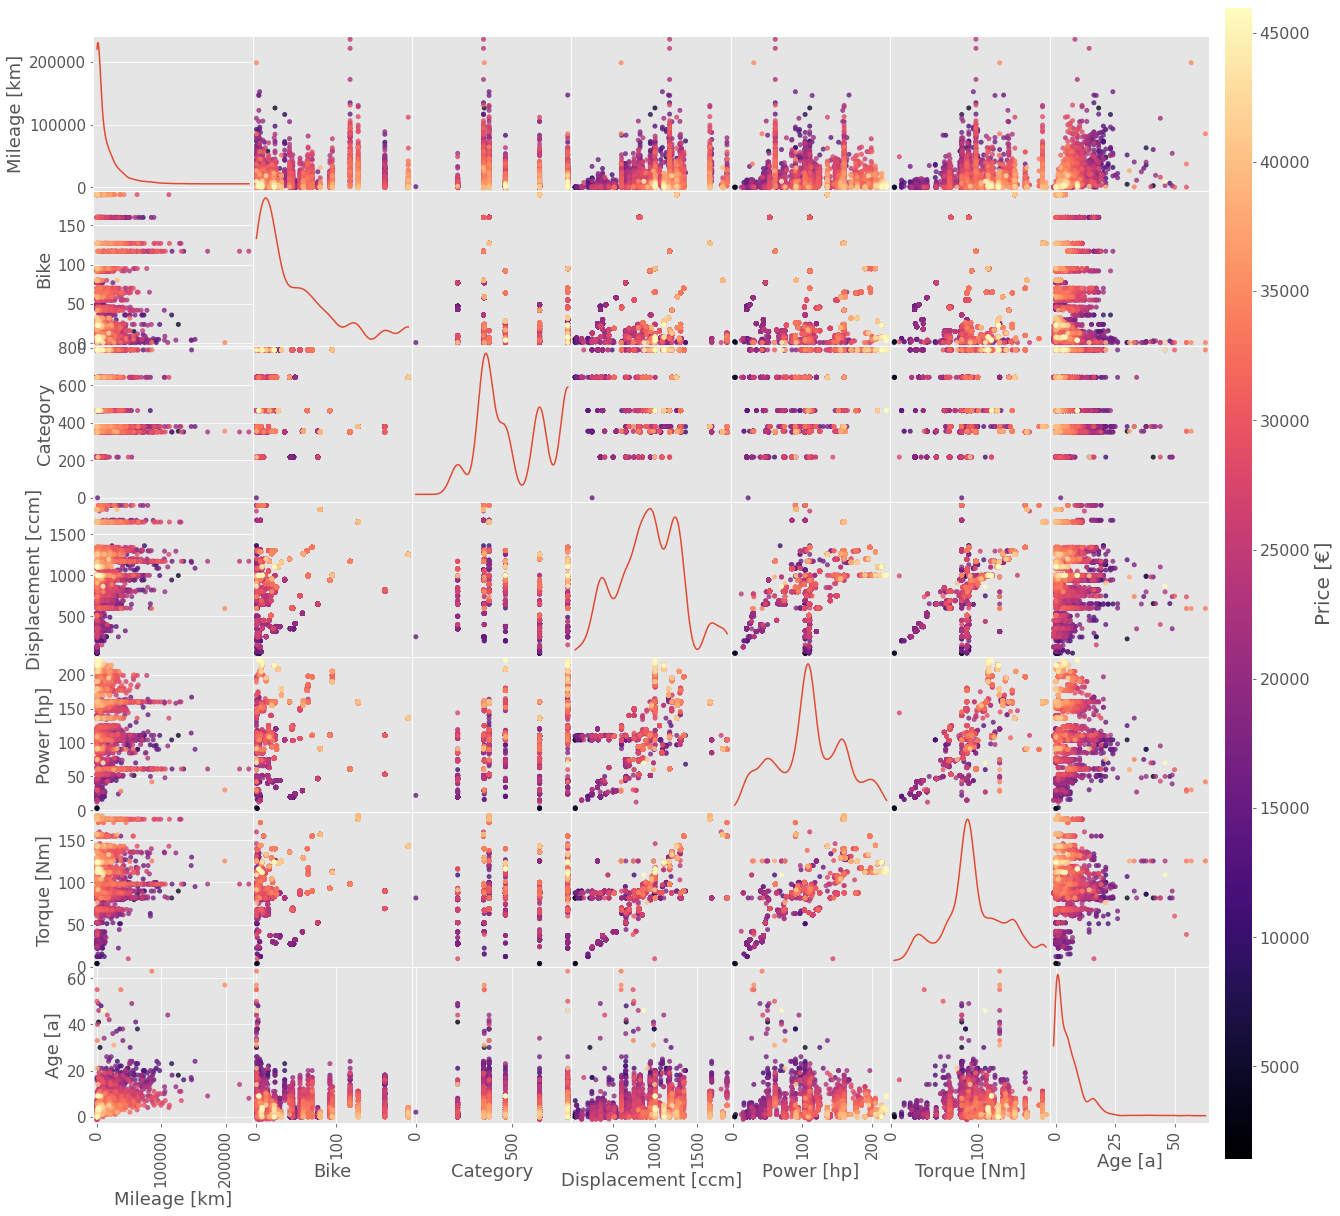
\includegraphics[width=\textwidth]{"content/pics/Scatter_Matrix_All.png"}
        \caption{Scatter Matrix of the input variables.}
        \label{fig:}
\end{figure}

\begin{figure}
    \centering
    \begin{subfigure}[b]{0.48\textwidth}
        \centering
        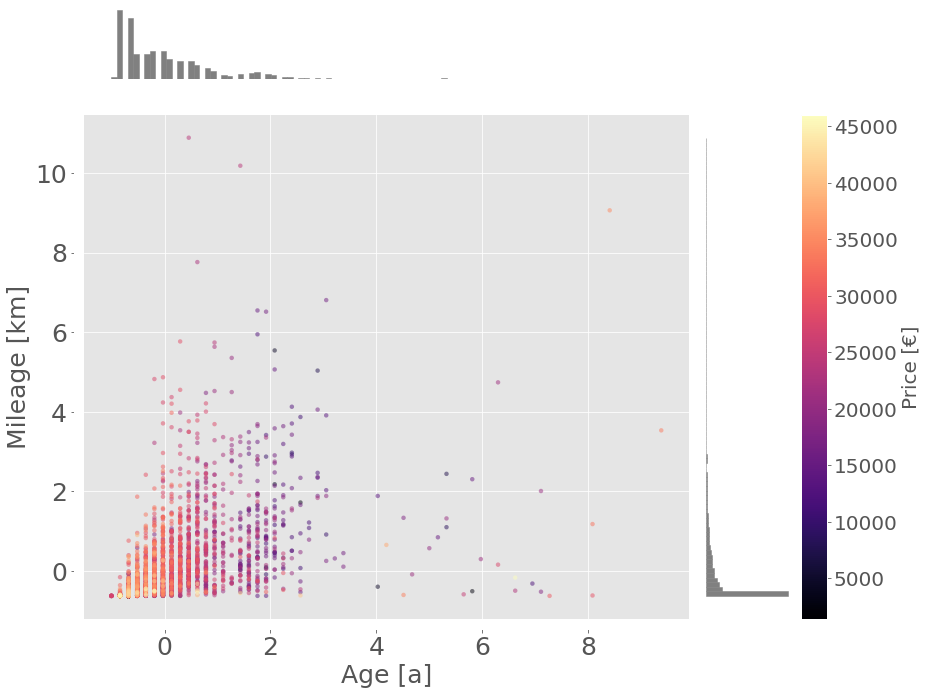
\includegraphics[width=\textwidth]{"content/pics/Scatter_Standard.png"}
        \caption{Standard Scaling.}
    \end{subfigure}
    \hfill
    \begin{subfigure}[b]{0.48\textwidth}
        \centering
        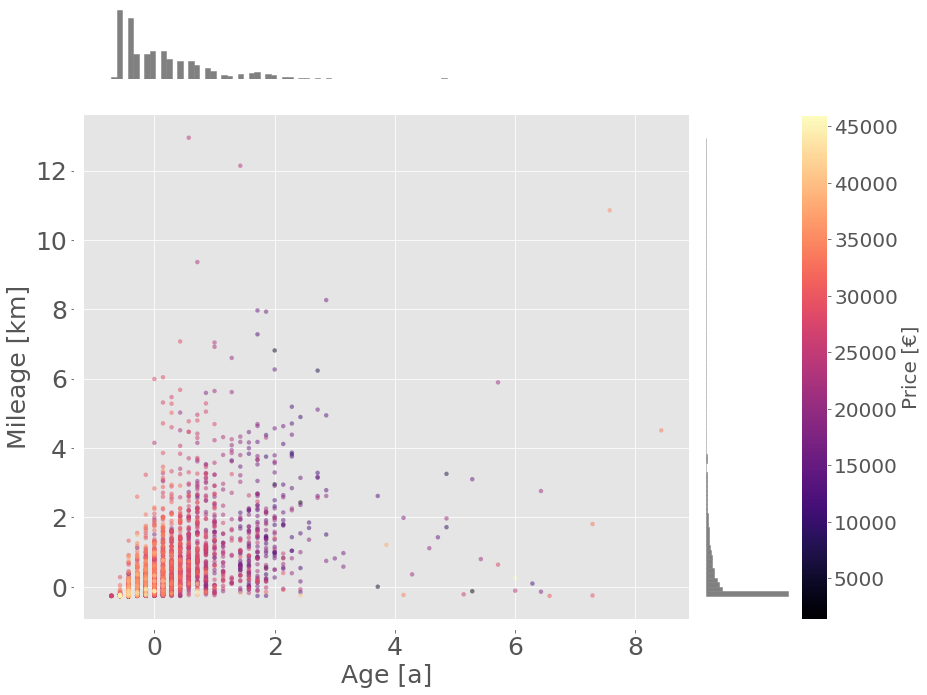
\includegraphics[width=\textwidth]{"content/pics/Scatter_Robust.png"}
        \caption{Robust Scaling.}
    \end{subfigure}
    \vfill 
    \begin{subfigure}[b]{0.48\textwidth}
        \centering
        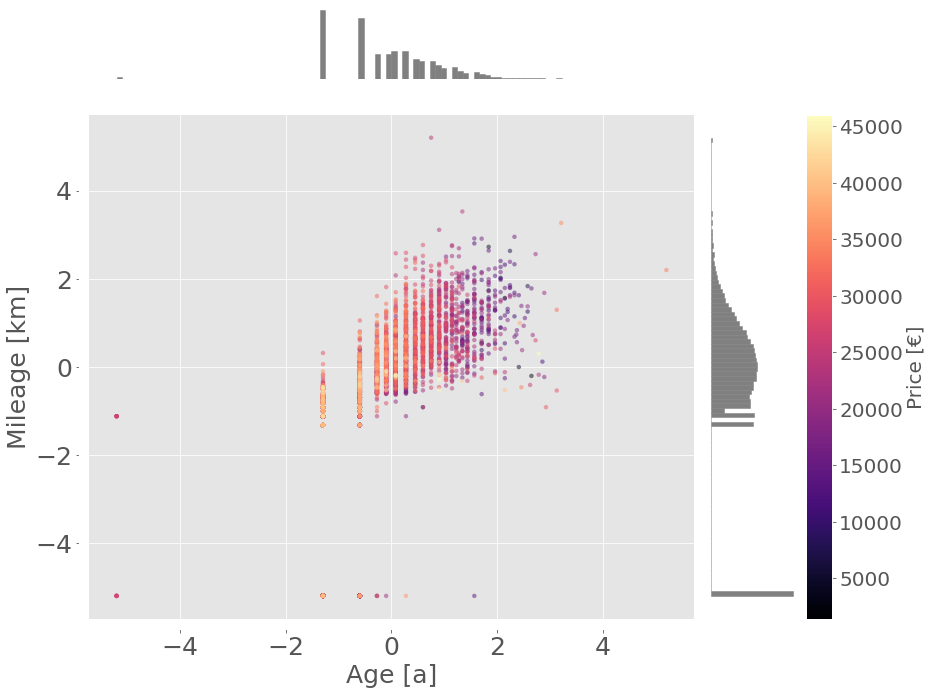
\includegraphics[width=\textwidth]{"content/pics/Scatter_Normal.png"}
        \caption{Gaussian Scaling.}
    \end{subfigure}
    \hfill
    \begin{subfigure}[b]{0.48\textwidth}
        \centering
        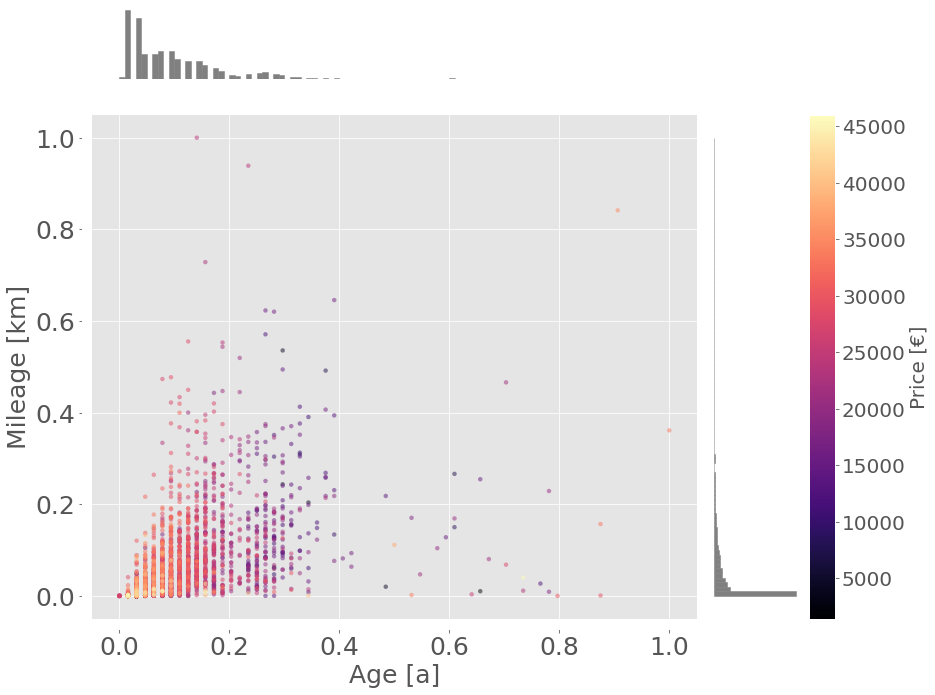
\includegraphics[width=\textwidth]{"content/pics/Scatter_MinMax.png"}
        \caption{Min-Max Scaling.}
    \end{subfigure}
    \vfill 
    \begin{subfigure}[b]{0.48\textwidth}
        \centering
        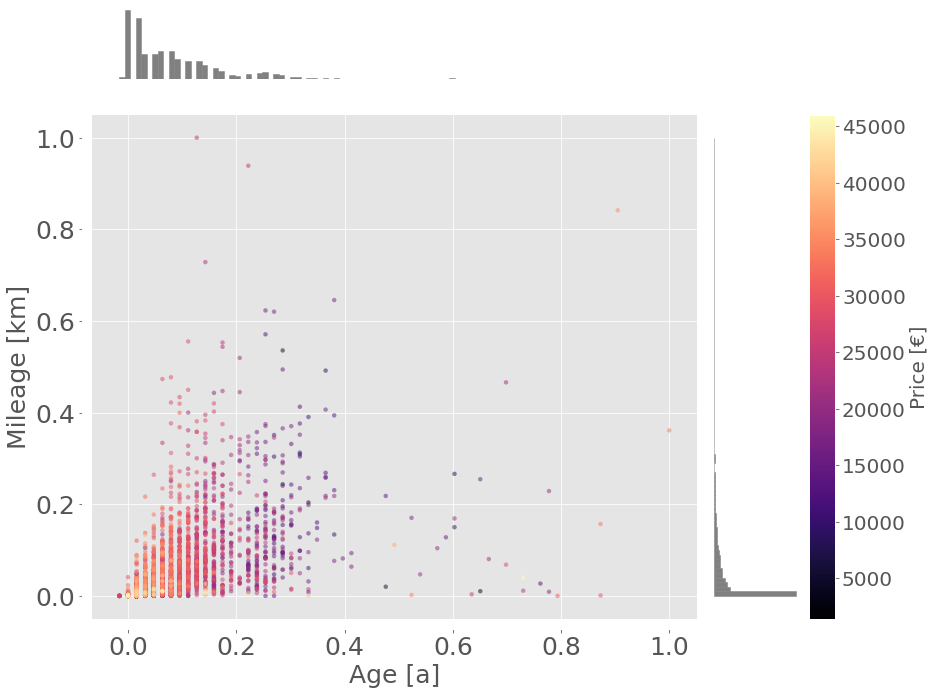
\includegraphics[width=\textwidth]{"content/pics/Scatter_MaxAbs.png"}
        \caption{Max-Abs Scaling.}
    \end{subfigure}
    \hfill
    \begin{subfigure}[b]{0.48\textwidth}
        \centering
        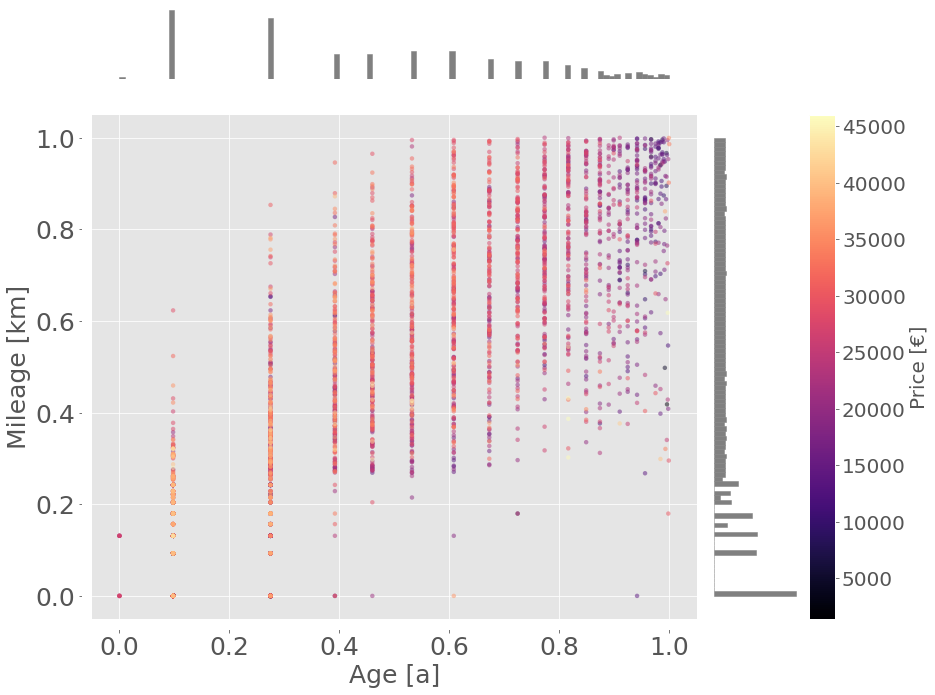
\includegraphics[width=\textwidth]{"content/pics/Scatter_Uniform.png"}
        \caption{Uniform Scaling.}
    \end{subfigure}
    \caption{Scatter plot of \textit{Mileage} and \textit{Age} with different scaling methods.}
    \label{fig:Scaling}
\end{figure}

\begin{figure}
    \centering
    \begin{subfigure}[h]{\textwidth}
        \centering
        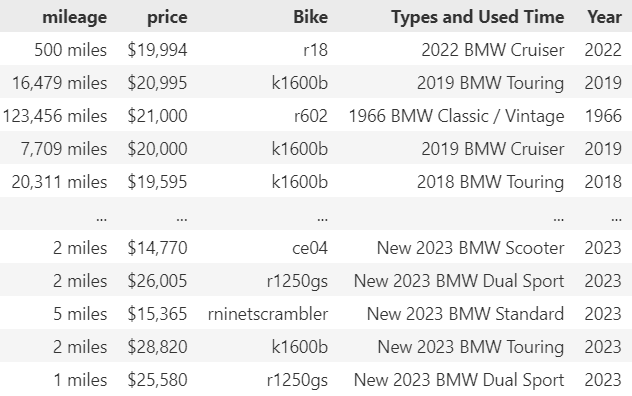
\includegraphics[width=\textwidth]{"content/pics/df_bmw_raw.png"}
    \end{subfigure}
    \vfill
    \begin{subfigure}[h]{\textwidth}
        \centering
        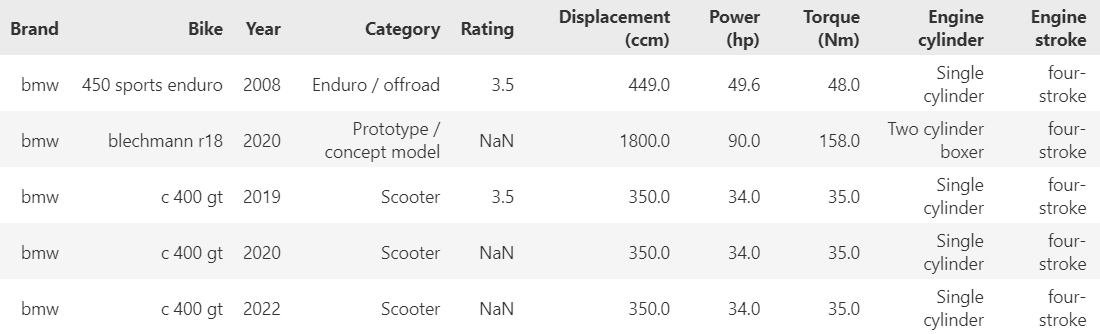
\includegraphics[width=\textwidth]{"content/pics/df_bikez_raw.png"}
    \end{subfigure}
    \caption{Excerpt of one of the datasets containing the price and selling specifications (upper) and the dataset
    containing the motorcycle specifications (lower).}
    \label{fig:Bike_Tables_raw}
\end{figure}

\begin{figure}
    \centering
    \begin{subfigure}[b]{0.48\textwidth}
        \centering
        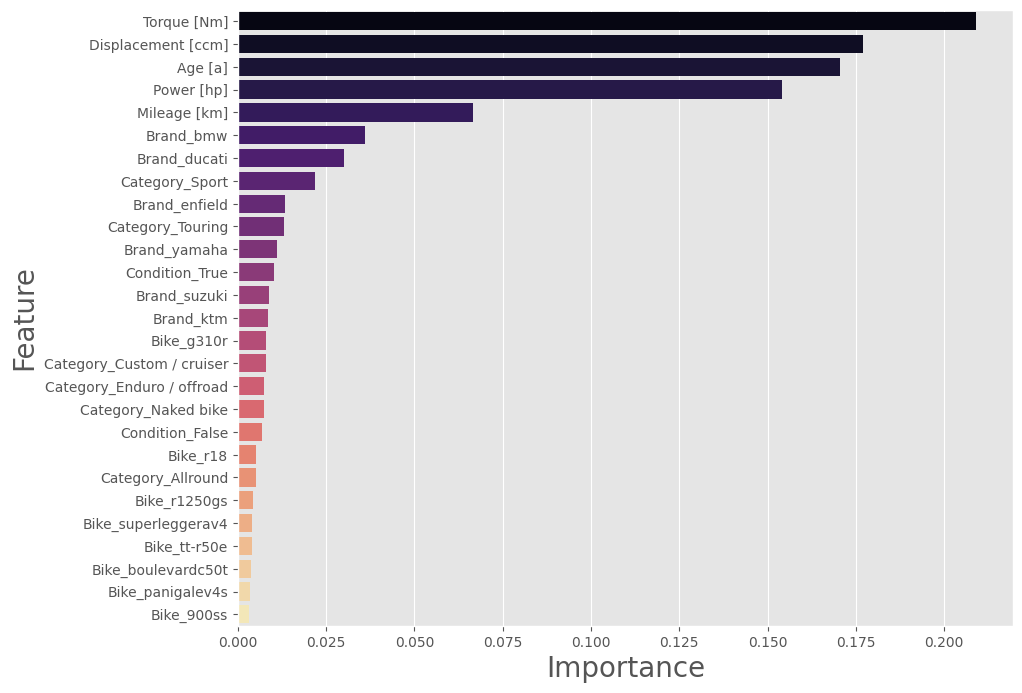
\includegraphics[width=\textwidth]{"content/pics/Feature_Importances_std.png"}
        \caption{Standard Scaling.}
    \end{subfigure}
    \hfill
    \begin{subfigure}[b]{0.48\textwidth}
        \centering
        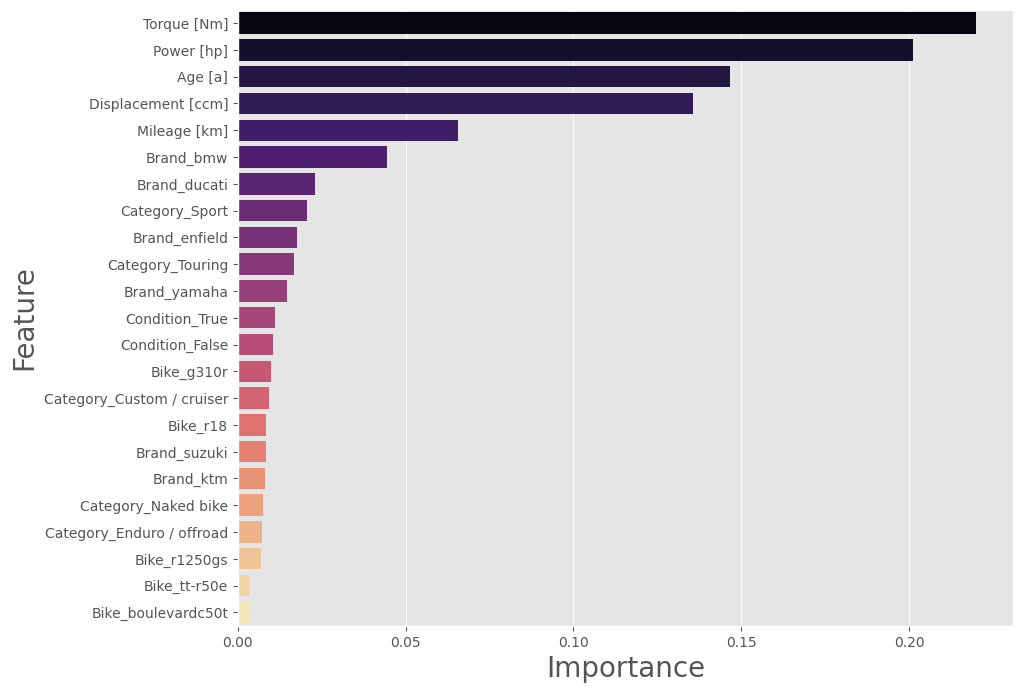
\includegraphics[width=\textwidth]{"content/pics/Feature_Importances_robust.png"}
        \caption{Robust Scaling.}
    \end{subfigure}
    \vfill 
    \begin{subfigure}[b]{0.48\textwidth}
        \centering
        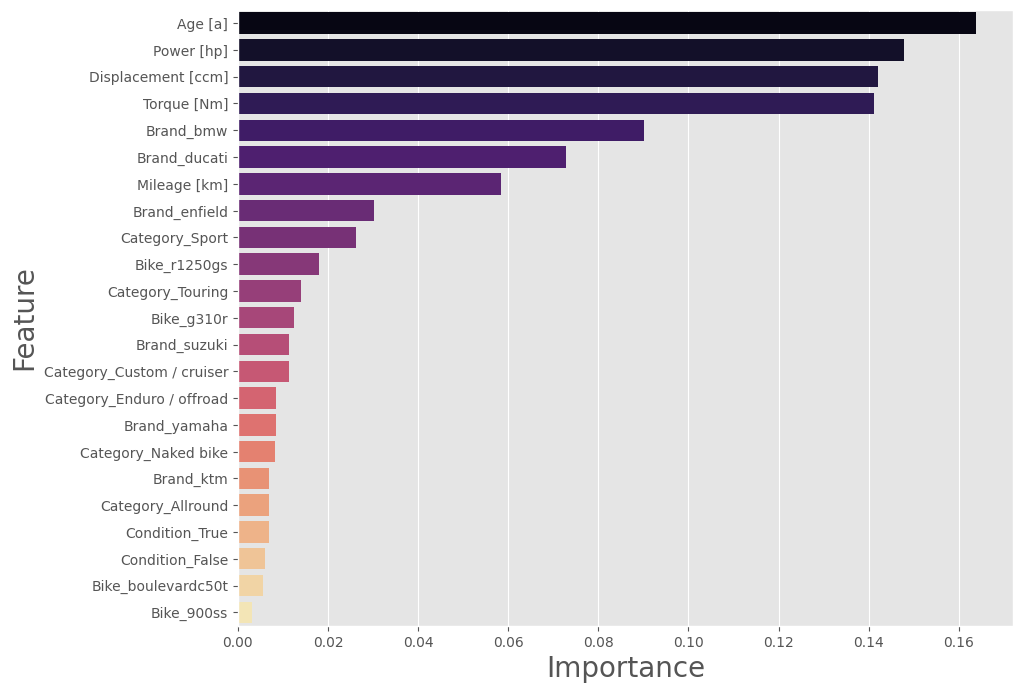
\includegraphics[width=\textwidth]{"content/pics/Feature_Importances_norm.png"}
        \caption{Gaussian Scaling.}
    \end{subfigure}
    \hfill
    \begin{subfigure}[b]{0.48\textwidth}
        \centering
        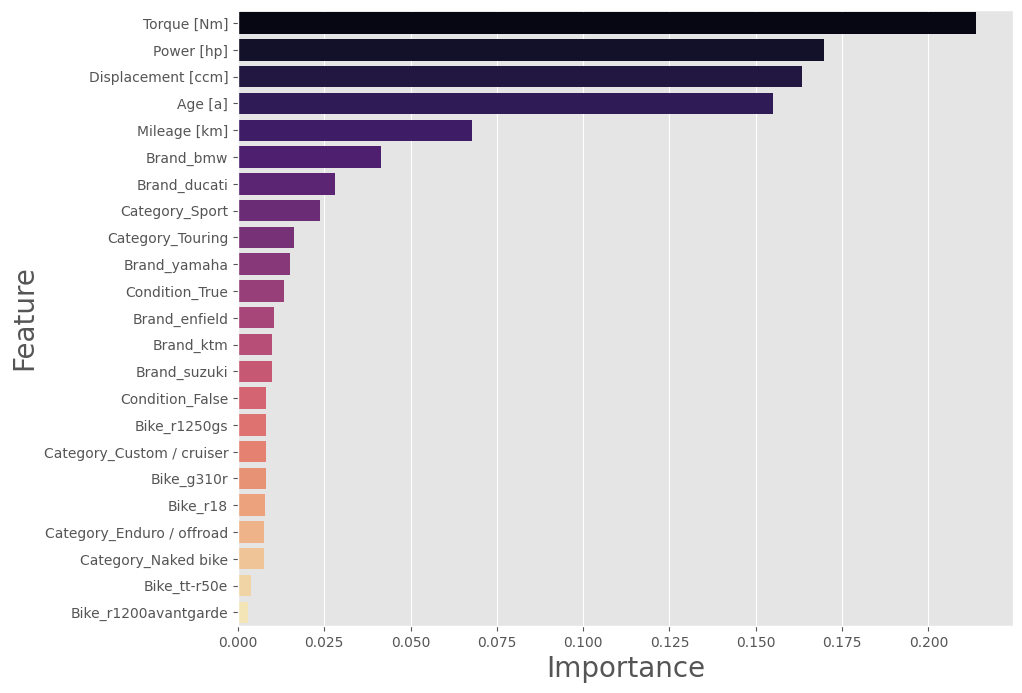
\includegraphics[width=\textwidth]{"content/pics/Feature_Importances_none.png"}
        \caption{No Scaling.}
    \end{subfigure}
    \caption{.}
    \label{fig:}
\end{figure}

\begin{figure}
    \centering
        \centering
        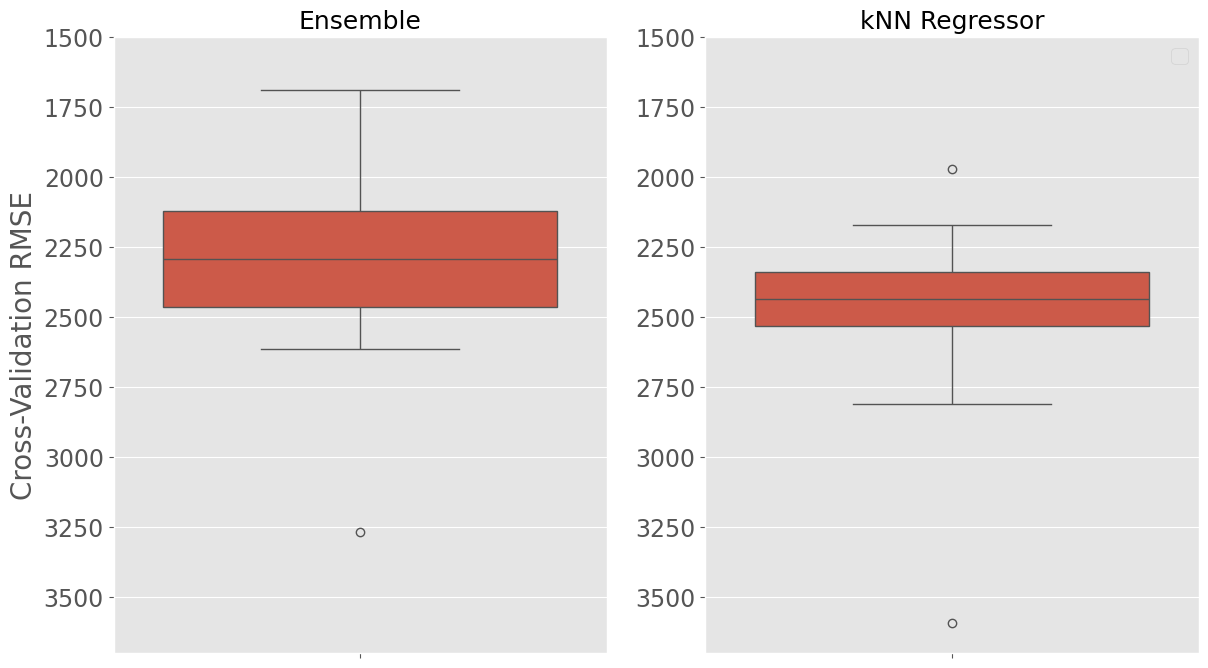
\includegraphics[width=\textwidth]{"content/pics/boxplots_crossval.png"}
        \caption{Box plots of the cross-validation results of the RMSE for the kNN regressor and the ensembled model.}
        \label{fig:}
\end{figure}

\begin{figure}
    \centering
        \centering
        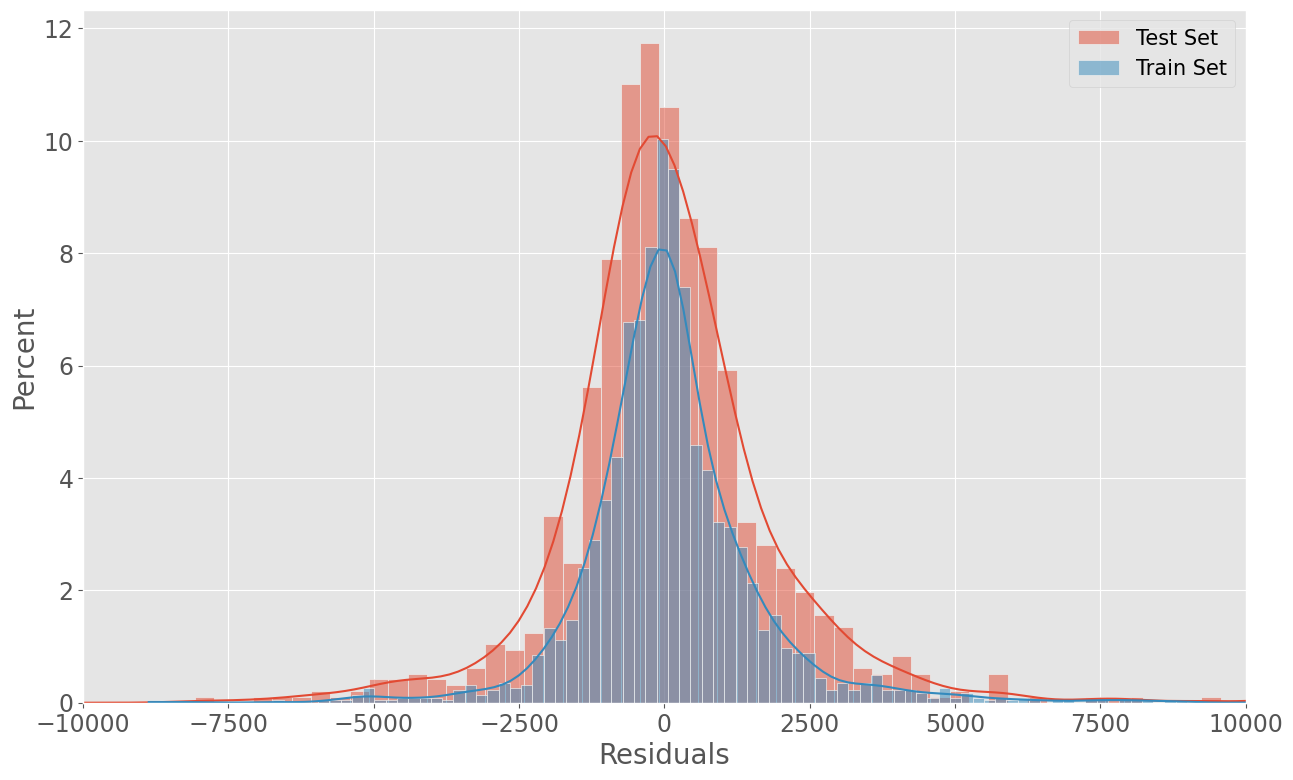
\includegraphics[width=\textwidth]{"content/pics/Distribution_Residuals.png"}
        \caption{Distribution of the residuals for the ensembled model for the training and testing subset.}
        \label{fig:}
\end{figure}
\begin{figure}
    \centering
        \centering
        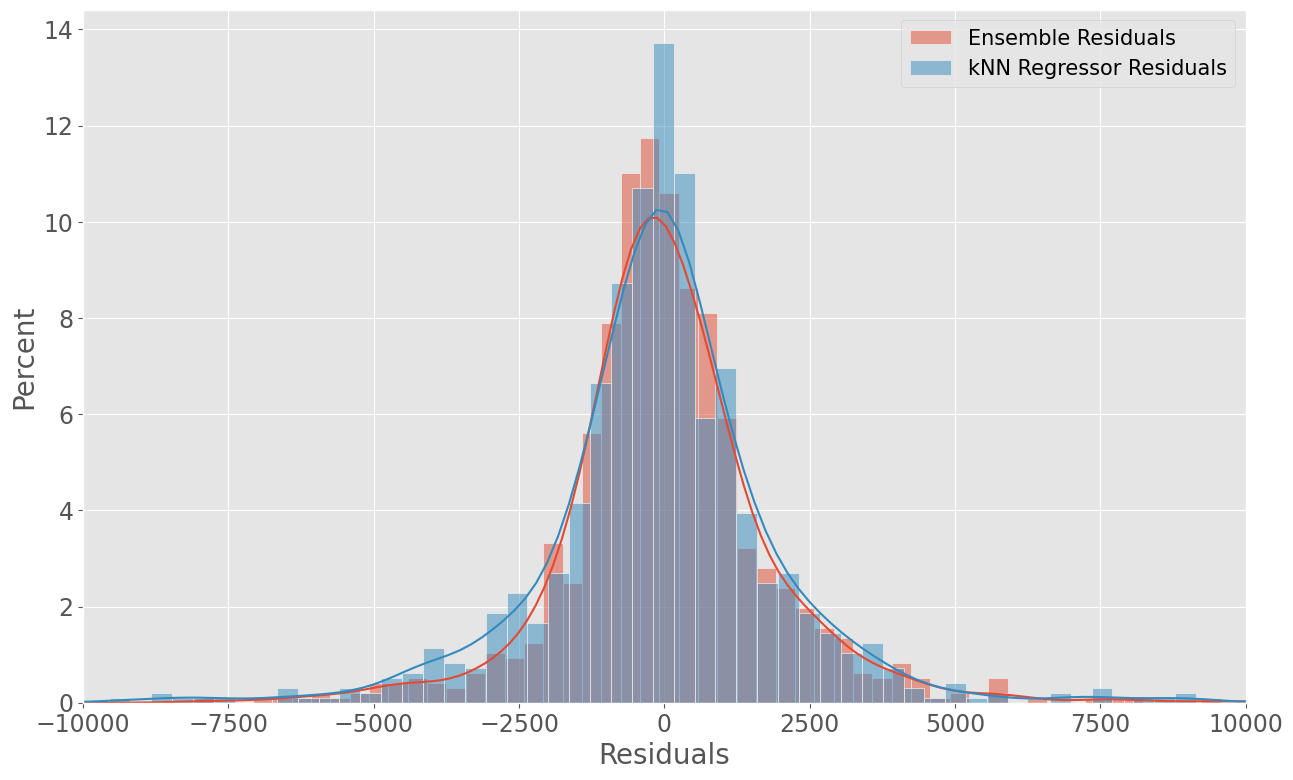
\includegraphics[width=\textwidth]{"content/pics/Distribution_Residuals_Ensemble_kNN.png"}
        \caption{Distribution of the residuals for the testing subset for the ensembled model and kNN regressor.}
        \label{fig:}
\end{figure}
\begin{figure}
    \centering
        \centering
        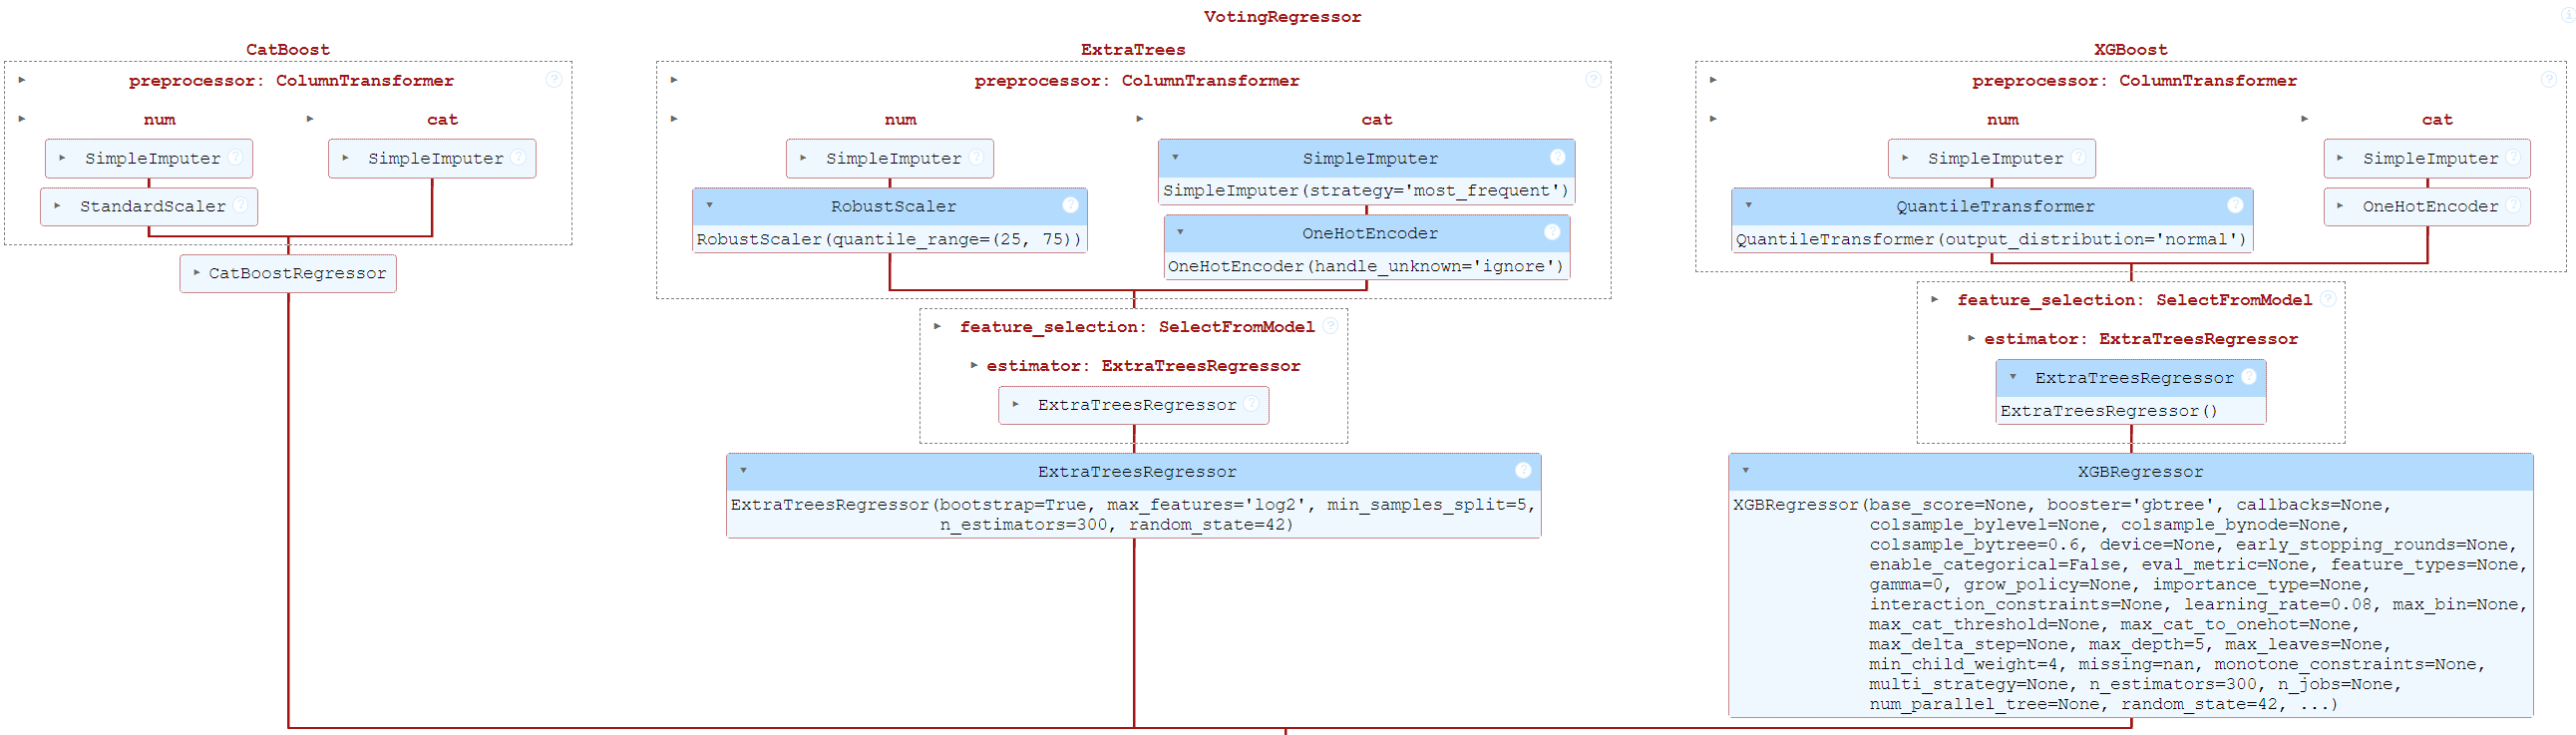
\includegraphics[width=\textwidth]{"content/pics/Ensembled_Model.png"}
        \caption{More detailed view of the model schematic of the ensembled model.}
        \label{fig:}
\end{figure}
\begin{figure}
    \centering
        \centering
        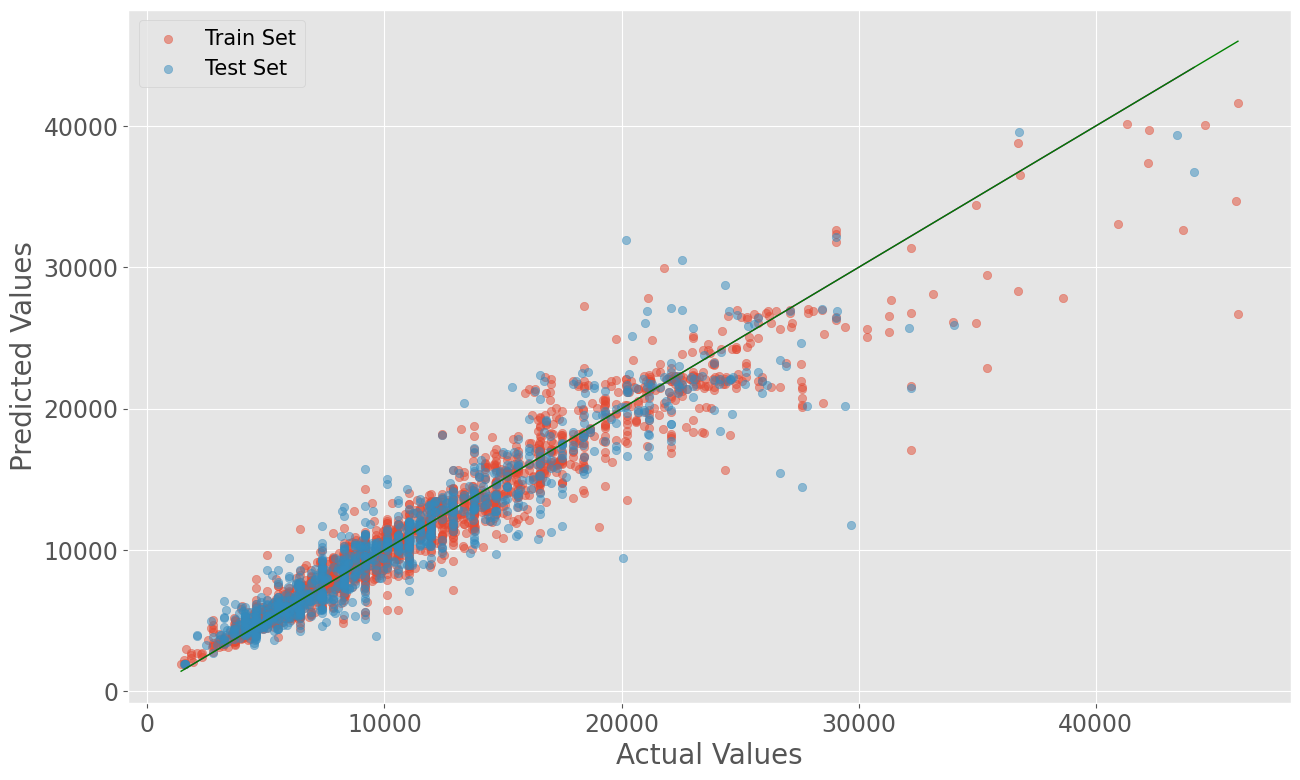
\includegraphics[width=\textwidth]{"content/pics/Predictionerrorplot.png"}
        \caption{Scatterplot of the true and predicted values for the training and testing subset for the ensembled model.}
        \label{fig:}
\end{figure}
\begin{figure}
    \centering
        \centering
        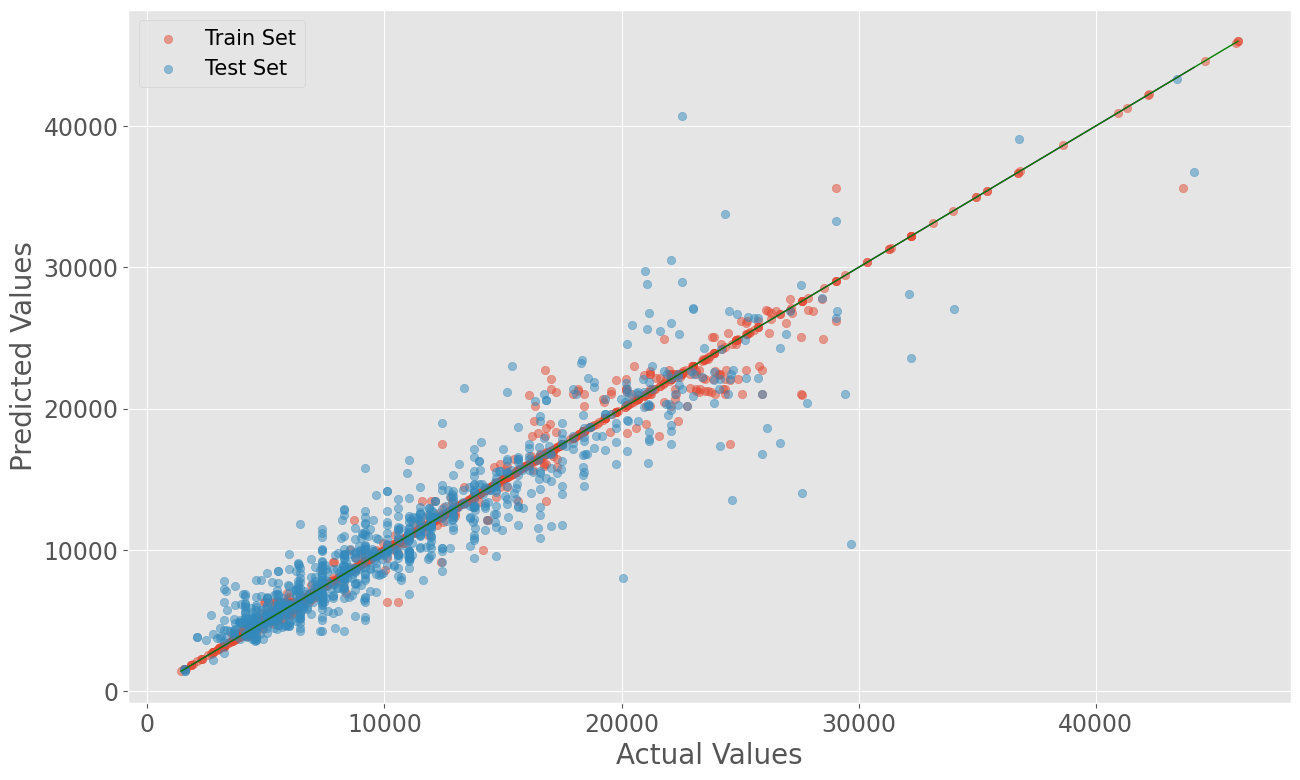
\includegraphics[width=\textwidth]{"content/pics/Predictionerrorplot_Knn.png"}
        \caption{Scatterplot of the true and predicted values for the training and testing subset for the kNN regressor.}
        \label{fig:}
\end{figure}
\begin{figure}
    \centering
        \centering
        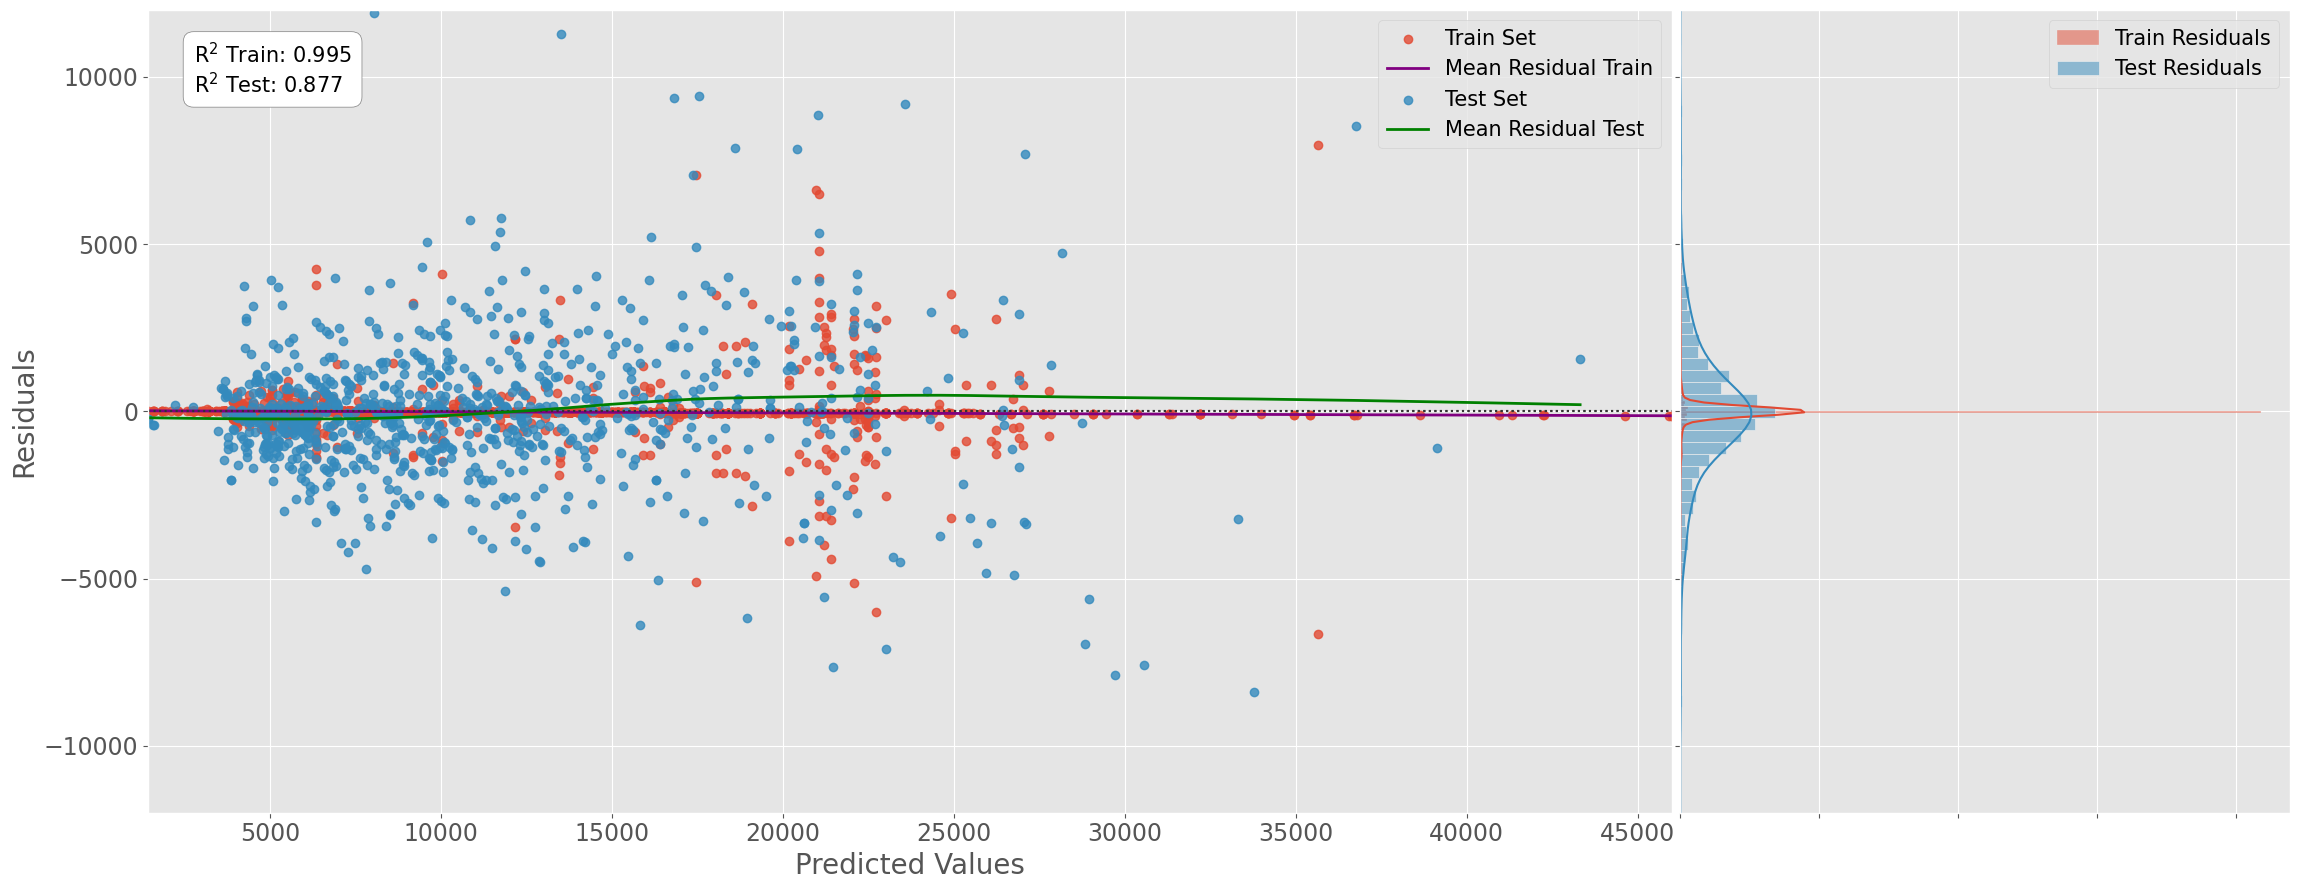
\includegraphics[width=\textwidth]{"content/pics/residuals_train_test_knn.png"}
        \caption{Scatter plot of the residuals for the training and testing subset of the kNN regressor.}
        \label{fig:}
\end{figure}
\begin{figure}[!]
    \centering
        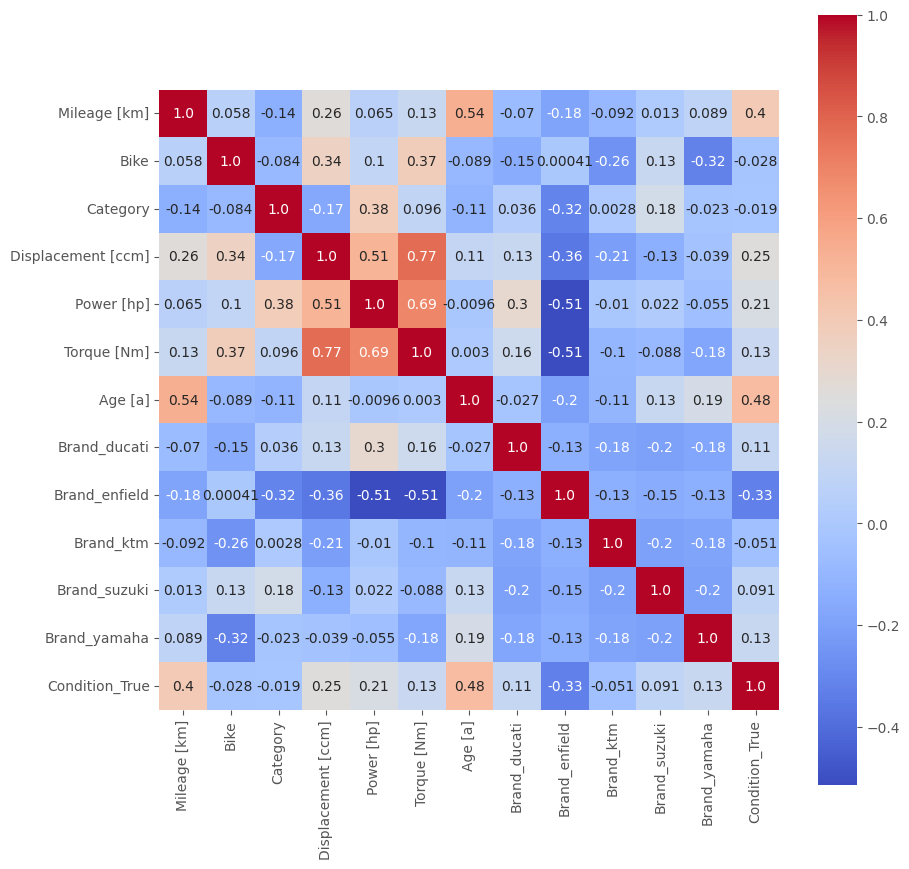
\includegraphics[width=1\textwidth]{"content/pics/correlation_matrix.png"}
        \caption{Correlation matrix of the used dataset attributes with encoded categorical columns.}
        \label{fig:}
\end{figure}